\section{物理量、函数与图像}
\subsection{先明确哪个量依赖哪个量}
把位置写成 $x(t)$，表示给定时间 $t$ 后可以确定位置；这里 $t$ 是自变量，$x$ 是因变量。函数关系不一定来自一个已经解出的显式公式，也可以来自几何约束、实验测量或动力学方程。开始计算前，应交代自变量范围、物理量正方向和参数的含义。例如绳长 $L$ 在一次运动中可视为固定参数，时间在变；若题目改为比较不同绳长的装置，$L$ 才成为另一个需要改变的量。

定义域是物理模型的一部分。小球尚未碰地时的自由落体公式不能直接延伸到碰地之后；液面高度必须非负；某个平方根的两个代数分支也未必都对应实际装配位置。几何图帮助确定允许范围，随后求导、积分和取极值都应在同一范围内进行。

函数图的横纵轴可以是不同物理量，因此纸面上的一个角度不直接等于具有量纲的变化率。设运动关系为 $x=L(t/\tau)^2$，其中 $L$ 为长度尺度、$\tau$ 为时间尺度。令 $s=t/\tau$，就有 $x/L=s^2$。图\ref{c1foundation:scales}左边使用物理坐标，右边使用无量纲坐标；二者表示同一过程，但横纵轴的刻度不同。
\fig{c1foundation:scales}{物理坐标与无量纲坐标表示同一变化关系}{\begin{tikzpicture}[scale=.8]
\begin{scope}
\draw[axis](0,0)--(3,0)node[right]{$t$};\draw[axis](0,0)--(0,3)node[above]{$x$};
\draw[world,domain=0:2.4,samples=50]plot(\x,{.45*\x*\x});
\draw[guide](1.8,0)node[below]{$\tau$}--(1.8,1.458)--(0,1.458)node[left]{$L$};
\node at(1.4,-.9){$x=L(t/\tau)^2$};
\end{scope}
\begin{scope}[xshift=5.7cm]
\draw[axis](0,0)--(3,0)node[right]{$t/\tau$};\draw[axis](0,0)--(0,3)node[above]{$x/L$};
\draw[world,domain=0:1.6,samples=50]plot(\x,{\x*\x});
\draw[guide](1,0)node[below]{$1$}--(1,1)--(0,1)node[left]{$1$};
\node at(1.4,-.9){同一过程的尺度表示};
\end{scope}
\end{tikzpicture}}

求速度时，$L,\tau$保持不变，而$s=t/\tau$随$t$变化。沿图\ref{c1foundation:scales}两套坐标之间的对应关系，链式法则给出
\[
v=\frac{\dd x}{\dd t}
=L\frac{\dd(s^2)}{\dd s}\frac{\dd s}{\dd t}
=L(2s)\frac1\tau
=\frac{2Lt}{\tau^2}.
\]
无量纲图上的导数$2s$不能直接当作有速度单位的$v$；必须乘回$L/\tau$。这一点会在坐标变换、实验图像斜率和近似展开中反复使用。

\subsection{平均变化与瞬时变化回答不同问题}
在有限时间$\Delta t\ne0$内，平均速度是$[x(t+\Delta t)-x(t)]/\Delta t$。对上面的二次位置函数，先展开有限增量：
\begin{align*}
\frac{x(t+\Delta t)-x(t)}{\Delta t}
&=\frac{L}{\tau^2}\frac{(t+\Delta t)^2-t^2}{\Delta t}\\
&=\frac{L}{\tau^2}\frac{2t\Delta t+(\Delta t)^2}{\Delta t}
=\frac{2Lt}{\tau^2}+\frac{L\Delta t}{\tau^2}.
\end{align*}
第二项来自有限时间内速度继续变化；只有令时间间隔趋零，才得到时刻$t$的瞬时速度。这个过程不是把分母直接写成零，而是先在非零间隔下整理，再取极限。

反过来，已知每个时刻的速度，要恢复一段过程的位移，需要累积 $v\,\dd t$，还要给出初始位置。导数、积分和初始条件各自提供不同信息：导数描述局部变化率，积分连接有限过程，初值确定常数。后文的严格定义将把这些图像变成可检验的计算，而不改变这里每个物理量与图中轴的对应。

% dedup-c1-knowledge
% thirty-c1-theory
\section{极限：从有限过程走向确定的结果}
\subsection{无限细分与收敛}
把长度为 $L_0$ 的线段反复对半分，每次保留其中一半，经过 $n$ 次操作后余长为 $L_n=L_0/2^n$。任何有限次操作都不能得到零长度，但这不妨碍余长以零为极限。极限描述的是“按同一规则继续下去，结果能否任意接近某个确定值”，并不要求某一步恰好等于该值。

数列 $a_n$ 收敛到 $A$，是指对任意给定的误差 $\varepsilon>0$，总能找到整数 $N$，使全部 $n>N$ 都满足 $|a_n-A|<\varepsilon$。这里“全部”很关键：偶尔接近并不能说明收敛。例如 $a_n=(-1)^n$ 在两个值之间往复跳动，不具有极限。几何级数则说明，无穷多段长度相加也可能得到有限值。当 $|q|<1$ 时，
\[
 S_N=a\frac{1-q^{N+1}}{1-q},\qquad
 \lim_{N\to\infty}S_N=\frac a{1-q}.
\]
先对有限项求和，再取极限，可以避免把无穷当作普通整数处理。

有限小数 $0.\underbrace{99\cdots9}_{n\text{ 位}}$ 等于 $1-10^{-n}$，它与一的差为 $10^{-n}$，趋于零。无限循环小数 $0.999\cdots$ 的定义正是这些有限截断值的极限，所以 $0.999\cdots=1$。这里每个截断值都小于一，但不能把有限截断值与无限小数所表示的实数混为一谈；极限等于一并不要求数列中某一项先达到一。

\fig{c1k-limit}{误差带要求后续全部项都留在带内}{\begin{tikzpicture}[x=.7cm,y=2.5cm]
\fill[blue!10](0,0)rectangle(8,.125);
\draw[axis](0,0)--(8.5,0)node[right]{$n$};
\draw[axis](0,0)--(0,1.12)node[above]{$L_n/L_0$};
\draw[guide](0,.125)--(8,.125)node[right]{$\varepsilon/L_0$};
\foreach \n in {0,...,8}{\fill(\n,{pow(.5,\n)})circle(1.4pt);}
\draw[guide](3,0)--(3,.7);\node[below]at(3,0){$N$};
\node at(5.5,.56){$n>N\Rightarrow L_n<\varepsilon$};
\end{tikzpicture}}
图 \ref{c1k-limit} 中的横线先由误差要求确定，再沿数列寻找进入误差带后不再离开的起点。减小允许误差，所需的起点可以向后移动，但产生数列的规则不变。因此证明收敛不是选取一个足够小的数值算一次，而是说明任意误差要求都能满足。若把公比改为 $q=-1/2$，各项虽在极限两侧交替，误差的绝对值仍按 $2^{-n}$ 衰减，也同样收敛。

\subsection{函数极限与左右极限}
当 $x$ 在定义域内趋近 $x_0$ 时，若 $f(x)$ 任意接近 $A$，记为 $\lim_{x\to x_0}f(x)=A$。严格地说，对任意 $\varepsilon>0$，存在 $\delta>0$，使 $0<|x-x_0|<\delta$ 时都有 $|f(x)-A|<\varepsilon$。条件中排除了 $x=x_0$，所以函数在该点未定义，也可能存在极限。

从两侧趋近得到同一个有限值，双侧有限极限才存在。若左侧趋于 $-\infty$、右侧趋于 $+\infty$，不能将二者合称一个有限极限。无穷远处的极限则考察 $|x|$ 很大时的行为；此时有理函数常可将分子、分母同时除以最高次幂，比较主导项。

已知两个有限极限后，可以相加、相乘；作商还要求分母极限非零。遇到 $0/0$，含义只是“直接代入不能决定结果”，应先因式分解、利用已知极限或建立上下界。不能把 $0/0$ 当作零，也不能不加条件地约去一个在整个邻域都可能为零的量。

极限值与函数值还应分开判断。例如 $f(x)=(x^2-a^2)/(x-a)$ 在 $x=a$ 处没有定义，但在 $x\ne a$ 时等于 $x+a$，因此极限为 $2a$。约去 $x-a$ 合法，是因为趋近过程排除了该点；它并没有给缺失点自动补上函数值。若另行规定 $f(a)=2a$，才得到连续延拓。物理近似中先化简再取极限，也必须保留这种定义域检查。

含多个小量时，还要先说明它们怎样趋近。例如细杆应变、摆角或折射角的近似，往往隐含其他参数保持不变。一个比值沿某种特殊关系趋近有确定结果，不能据此断言所有趋近方式都给出同一极限。先固定参数，再处理自变量，能避免把不同的物理过程混成一个数学极限。


图\ref{c1deep:hole}把两种容易混淆的情形并列起来。左图中，曲线在 $x=a$ 两侧都走向空心点 $H$；把实际函数值另定在 $K$，只改变一个点，不改变极限。连续则还要求 $K$ 与 $H$ 重合。右图中，两支分别走向不同高度 $A_-$、$A_+$，无论怎样补上中心点，都不能使双侧极限存在。因此处理分段函数时，应沿曲线分别走到接点，再比较两侧高度，最后才检查接点本身。
\fig{c1deep:hole}{邻近点的趋向决定极限，中心点的取值决定能否连续}{\begin{tikzpicture}[scale=.88]
\begin{scope}
\draw[axis](0,0)--(4,0)node[right]{$x$};\draw[axis](0,0)--(0,3.2)node[above]{$f$};
\draw[blue,thick](.3,.7)--(3.5,2.3);\draw[guide](2,0)--(2,2.9);
\fill[white](2,1.55)circle(2.7pt);\draw[blue](2,1.55)circle(2.7pt);\node[below right]at(2,1.55){$H:(a,A)$};
\fill(2,2.7)circle(2pt)node[above]{$K:(a,f(a))$};\node[below]at(2,0){$a$};
\draw[flow,blue](.6,.85)--(1.35,1.225);\draw[flow,blue](3.3,2.2)--(2.6,1.85);
\node at(2,-.8){极限存在，函数可不连续};
\end{scope}
\begin{scope}[xshift=5.5cm]
\draw[axis](0,0)--(4,0)node[right]{$x$};\draw[axis](0,0)--(0,3.2)node[above]{$f$};
\draw[blue,thick](.3,.55)--(2,1.1);\draw[red,thick](2,2.1)--(3.6,2.7);
\draw[guide](2,0)--(2,3);\draw[blue,fill=white](2,1.1)circle(2pt);\draw[red,fill=white](2,2.1)circle(2pt);
\node[right]at(2,1.1){$A_-$};\node[left]at(2,2.1){$A_+$};\node[below]at(2,0){$a$};
\node at(2,-.8){左右极限不相等};
\end{scope}
\end{tikzpicture}}


\subsection{从误差要求反求自变量的范围}
极限中的“足够接近”应由误差要求决定。以 $f(x)=x^2$在 $x=a$处为例，要使 $|x^2-a^2|<\varepsilon$，先分解为 $|x-a||x+a|$。若同时限制 $|x-a|<1$，三角不等式给出 $|x+a|\le|x-a|+2|a|<1+2|a|$。因此取
\[\delta=\min\left\{1,\frac{\varepsilon}{1+2|a|}\right\},\]
便能保证 $0<|x-a|<\delta$时 $|x^2-a^2|<\varepsilon$。这里先给变化系数一个统一上界，再反求允许的输入误差，完成了从定性接近到定量控制的转换。$a=0$也被同一证明包含；若单独利用 $|x^2|=|x|^2$，则可以取得更宽的范围 $\delta=\sqrt\varepsilon$。

图\ref{c1k-window}中先给出竖直误差带，再寻找横向区间，使曲线在该区间的全部点都留在带内。所找区间可以比实际允许的区间小，证明并不要求 $\delta$最大。函数在中心点是否定义，与去心邻域内的极限是两件事；因此 $\sin x/x$在零点没有定义，仍可有确定的零点极限。
\fig{c1k-window}{竖直误差带限制一段完整的横向邻域}{\begin{tikzpicture}[x=1.4cm,y=.7cm]
\fill[blue!8](0,1.05)rectangle(3.2,3.45);
\draw[axis](0,0)--(3.6,0)node[right]{$x$};\draw[axis](0,0)--(0,4.3)node[above]{$f(x)$};
\draw[world]plot[domain=.3:2,samples=60]({\x},{(\x)^2});
\draw[guide](0,1.05)--(3.2,1.05) (0,3.45)--(3.2,3.45);
\draw[guide](1.2,0)--(1.2,3.45) (1.8,0)--(1.8,3.45);
\fill(1.5,2.25)circle(1.3pt)node[above left,fill=white,inner sep=1pt]{$(a,f(a))$};
\node[below left]at(1.2,0){$a-\delta$};\node[below right]at(1.8,0){$a+\delta$};
\node[right]at(3.2,3.45){$f(a)+\varepsilon$};\node[right]at(3.2,1.05){$f(a)-\varepsilon$};
\end{tikzpicture}}

\subsection{三角极限的几何依据}
三角函数求导所用的基本极限，可以直接由单位圆的面积比较建立。图\ref{fv:c1:sine}取 $0<h<\pi/2$，$OA=OB=1$，$AT$为圆的切线。三角形 $OAB$包含在扇形 $OAB$内，扇形又包含在三角形 $OAT$内，因此
\[
 \tfrac12\sin h<\tfrac12h<\tfrac12\tan h,
 \qquad \cos h<\frac{\sin h}{h}<1.
\]
\fig{fv:c1:sine}{以弧度表示扇形面积，才能把几何夹逼写成极限}{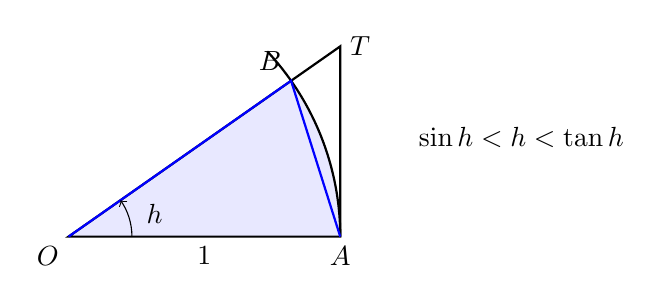
\begin{tikzpicture}[scale=1.15]
\coordinate(O)at(0,0);\coordinate(A)at(3,0);\coordinate(B)at(2.457,1.721);\coordinate(T)at(3,2.101);
\fill[blue!9](O)--(A)arc(0:35:3)--cycle;
\draw[thick](O)--(A)--(T)--cycle;\draw[thick](A)arc(0:43:3);\draw[blue,thick](O)--(B)--(A);
\draw[->](.7,0)arc(0:35:.7);\node at(.95,.25){$h$};
\node[below left]at(O){$O$};\node[below]at(A){$A$};\node[above left]at(B){$B$};\node[right]at(T){$T$};
\node[below]at(1.5,0){$1$};\node at(5,1.1){$\sin h<h<\tan h$};
\end{tikzpicture}}
当 $h\to0^+$，两端均趋于一；$\sin h/h$是偶函数，左极限相同，故极限为一。图中的 $h$必须是弧度数，否则扇形面积不等于 $h/2$。同时 $(1-\cos h)/h=\sin^2h/[h(1+\cos h)]\to0$，于是求导推导所需的两个极限都有了依据。

利用同一极限，还可把二阶小量写成可判断的形式：
\[
 \frac{1-\cos h}{h^2}
 =\frac12\left(\frac{\sin(h/2)}{h/2}\right)^2\longrightarrow\frac12.
\]
因此 $\sin h$ 的首项是 $h$，$1-\cos h$ 的首项是 $h^2/2$。前者不能用来抵消后者的二阶分母；先辨认小量的阶次，才能选择合法的化简。这里的近似是在 $h\to0$ 时成立，图\ref{fv:c1:sine}并没有断言有限角度下弧长与弦长相等。


\section{导数与微分}
\subsection{割线极限和局部线性关系}
设 $y=f(x)$。从 $P(x,f(x))$ 到邻近点 $Q(x+h,f(x+h))$ 的割线斜率是
\[
 \frac{\Delta y}{h}=\frac{f(x+h)-f(x)}h.
\]
若 $h\to0$ 时该比值具有有限极限，就定义
\[
 f'(x)=\lim_{h\to0}\frac{f(x+h)-f(x)}h.
\]
对坐标单位固定的函数图像，导数给出切线斜率。对物理量关系，它给出瞬时变化率，并带有相应单位：$\dd x/\dd t$ 的单位为速度，$\dd v/\dd t$ 的单位为加速度。画图时改变横纵坐标的缩放会改变纸面夹角，但不会改变物理变化率。

可导也可以写成局部线性形式
\[
 f(x+h)=f(x)+f'(x)h+o(h),\qquad
 \lim_{h\to0}\frac{o(h)}h=0.
\]
取 $\dd x=h$，定义 $\dd y=f'(x)\dd x$。$\dd y$ 是增量 $\Delta y$ 的线性部分，而非对任意有限 $h$ 都有 $\Delta y=\dd y$。例如 $y=x^2$ 时，
\[
 \Delta y=2x h+h^2,\qquad \dd y=2x\,\dd x.
\]
这一区分将决定近似展开应保留到哪一阶。

局部线性式还说明可导必连续：当 $h\to0$时，$f'(x)h$与 $o(h)$均趋零，故 $f(x+h)-f(x)\to0$。反过来，连续只限制增量本身，不保证差商具有唯一极限。下面先借切线图理解局部线性关系，再分别检查连续、一阶可导与二阶可导。

\fig{c1k-tangent}{曲线增量与切线增量具有不同的二阶部分}{\begin{tikzpicture}[scale=.95]
\draw[axis](0,0)--(3.1,0)node[right]{$x$};
\draw[axis](0,0)--(0,4.6)node[above]{$y$};
\draw[world,domain=.25:2.1,samples=40]plot(\x,{\x*\x});
\draw[blue](1,1)--(2,4);
\draw[red,domain=.5:2.5]plot(\x,{2*\x-1});
\fill(1,1)circle(1.6pt)node[left]{$P$};\fill(2,4)circle(1.6pt)node[right]{$Q$};
\fill(2,3)circle(1.3pt)node[right]{$T$};
\draw[guide](1,1)--(2,1)--(2,4);
\draw[dim](1,.65)--(2,.65)node[midway,below]{$h$};
\draw[dim](2.4,1)--(2.4,4)node[midway,right]{$\Delta y$};
\draw[dim,red](3.3,1)--(3.3,3)node[midway,right]{$\dd y$};
\end{tikzpicture}}
图 \ref{c1k-tangent} 取 $y=x^2$、$P=(1,1)$，$Q$ 在曲线上，$T$ 在切线上，且 $Q,T$ 的横坐标相同。由 $P$ 的高度到 $Q$ 的高度是实际增量 $2h+h^2$，到 $T$ 的高度是线性增量 $2h$。二者绝对差为 $h^2$，相对于一阶项又小一个 $h$ 的量级。图中为了看清差别取了较大的间隔；当 $h$ 缩小时，这一构图说明微分为什么能作局部近似，也说明它为什么不能直接代替有限变化。

在测量误差估计中，同样可用 $\Delta y\simeq f'(x)\Delta x$，但要保证误差区间内的导数变化不显著。若 $f'(x)=0$，一阶估计只说明线性项消失，不能说明测量误差完全不影响结果，此时应继续检查二阶项。


\subsection{连续、可导与二次可导的图像区别}
图\ref{c1deep:smooth}中的三张图依次对应 $f(x)=|x|$、$g(x)=x|x|$ 和 $g'(x)=2|x|$。左图的两条割线在零点停留于斜率 $-1$ 和 $1$，所以曲线虽然接上，却没有唯一切线。中图的两侧斜率都趋于零，故零点有水平切线；右图说明它的导函数仍有折角，所以二阶导数不存在。判断“光滑”必须说清正在讨论哪一阶导数。
\fig{c1deep:smooth}{函数接上、切线接上与导函数可导是逐级增加的要求}{\begin{tikzpicture}[scale=.8]
\begin{scope}\draw[axis](-1.6,0)--(1.6,0)node[right]{$x$};\draw[axis](0,-.3)--(0,2)node[above]{$f$};
\draw[blue,thick](-1.3,1.3)--(0,0)--(1.3,1.3);\node at(0,-.85){$|x|$：折角};\node[left]at(-.7,.8){$-1$};\node[right]at(.7,.8){$+1$};\end{scope}
\begin{scope}[xshift=4.3cm]\draw[axis](-1.6,0)--(1.6,0)node[right]{$x$};\draw[axis](0,-1.5)--(0,2)node[above]{$g$};
\draw[blue,thick,domain=-1.1:1.1,samples=60]plot(\x,{\x*abs(\x)});\draw[red,thick](-1.3,0)--(1.3,0);\node at(0,-2){$x|x|$：切线相同};\end{scope}
\begin{scope}[xshift=8.6cm]\draw[axis](-1.6,0)--(1.6,0)node[right]{$x$};\draw[axis](0,-.3)--(0,2.7)node[above]{$g'$};
\draw[blue,thick](-1.1,2.2)--(0,0)--(1.1,2.2);\node at(0,-.85){$2|x|$：再现折角};\end{scope}
\end{tikzpicture}}
计算时，这三张图对应三个不同检验：先比较 $f(x)$ 与 $f(0)$，再比较两侧差商，最后检查导函数的差商。图像帮助定位可疑点，存在性仍由极限决定。碰撞前后的位移可以连续，速度却发生突变；这正是“函数连续但不可导”的物理情形，不能跨过碰撞时刻沿用同一光滑运动公式。


\subsection{基本函数的导数怎样得到}
对正整数 $n$，二项式展开给出
\[
 \frac{(x+h)^n-x^n}h
 =nx^{n-1}+\binom n2 x^{n-2}h+\cdots,
\]
取极限得到 $(x^n)'=nx^{n-1}$。一般实数幂在其可导的实数定义区间内仍满足这个规律，例如 $x>0$ 时 $(\sqrt x)'=1/(2\sqrt x)$。

三角函数求导使用弧度制。由 $\lim_{h\to0}\sin h/h=1$ 及
$(1-\cos h)/h\to0$，
\[
 \frac{\sin(x+h)-\sin x}h
 =\sin x\frac{\cos h-1}h+\cos x\frac{\sin h}h
 \longrightarrow\cos x.
\]
余弦同样先展开角和，再对两个商取极限：
\[
 \frac{\cos(x+h)-\cos x}{h}
 =\cos x\frac{\cos h-1}{h}-\sin x\frac{\sin h}{h}
 \longrightarrow-\sin x.
\]
所以 $(\cos x)'=-\sin x$。若角度以度为数值，必须补上弧度换算因子，不能直接套用这些式子。

指数函数的导数也可从局部增量理解。由指数的乘法性质，
\[
 \frac{\e^{x+h}-\e^x}{h}
 =\e^x\frac{\e^h-1}{h}.
\]
自然底数 $\e$ 的特征是最后一个比值在 $h\to0$ 时趋于一，因此 $(\e^x)'=\e^x$。换成底数 $a>0$ 时，$a^x=\e^{x\ln a}$，还会出现系数 $\ln a$。这解释了为什么用自然指数表示连续增长，方程中最少出现额外系数。

再把自然对数看成指数的反函数。若 $y=\ln x$，则 $x=\e^y$。对同一个自变量 $x$ 求导，左侧导数为一，右侧须经过中间变量 $y$，于是
$1=\e^y\,\dd y/\dd x=x\,\dd y/\dd x$，得到 $(\ln x)'=1/x$，要求 $x>0$。在负半轴，$\ln|x|=\ln(-x)$，链式法则给出 $(\ln(-x))'=(-1)/(-x)=1/x$；因此在不跨越零点的区间内统一写成 $(\ln|x|)'=1/x$。

求导公式中的定义区间必须随函数一同保留。例如 $\sqrt{x}$ 在 $x=0$ 有函数值，右侧差商却为 $1/\sqrt h$，不能得到有限的右导数；因此写出 $1/(2\sqrt x)$ 后，不能把 $x=0$ 当作普通代入点。又如对数只允许正的自变量，$\ln|x|$ 虽能统一两侧公式，零点仍是断开的边界。

三角函数在物理中通常以 $\theta=\omega t+\phi$ 为自变量。先对角度求导，再对时间求导，会带来频率因子 $\omega$；再求一次还会再出现一个 $\omega$。由此得到的速度振幅与加速度振幅分别具有长度每时间、长度每时间平方的单位，这同时是检验求导系数是否遗漏的有效办法。

\subsection{乘积、商与复合函数}
设 $u,v$ 均可导。在乘积增量中加减 $u(x+h)v(x)$，便有
\[
 \Delta(uv)=v(x)\Delta u+u(x)\Delta v+\Delta u\,\Delta v.
\]
除以 $h$ 后，最后一项趋于零，于是
\[
 (uv)'=u'v+uv',\qquad
 \left(\frac uv\right)'=\frac{u'v-uv'}{v^2}\quad(v\ne0).
\]
这表明乘积的变化来自两个因子的共同变化，不等于两个导数的乘积；取 $v=1$检查，就能立即排除误写的 $u'v'$。


图\ref{c1deep:product}把乘积 $uv$ 看成矩形面积。对正的 $u,v$ 和正增量，面积增加由三块组成：沿右边增加的条带为 $v\Delta u$，沿上边增加的条带为 $u\Delta v$，右上角小块为 $\Delta u\Delta v$。当两个增量都与 $h$ 同阶时，小角块是二阶量；先除以 $h$ 再取极限，它才消失。不能在有限变化时直接把这块面积漏掉。带符号的增量仍满足前面的代数恒等式，图中的正增量只是便于辨认各项。
\fig{c1deep:product}{乘积的两项一阶变化来自两条边，各因子不能同时求导后相乘}{\begin{tikzpicture}
\fill[gray!10](0,0)rectangle(4,2.2);\fill[blue!16](4,0)rectangle(5.2,2.2);\fill[red!14](0,2.2)rectangle(4,3.1);\fill[orange!25](4,2.2)rectangle(5.2,3.1);
\draw[thick](0,0)rectangle(5.2,3.1);\draw(4,0)--(4,3.1) (0,2.2)--(5.2,2.2);
\node at(2,1.1){$uv$};\node at(4.6,1.1){$v\Delta u$};\node at(2,2.65){$u\Delta v$};
\draw[->](6.5,3.6)--(4.6,2.65);\node[above]at(6.2,3.6){$\Delta u\Delta v$};
\draw[dim](0,-.4)--(4,-.4)node[midway,below]{$u$};\draw[dim](4,-.4)--(5.2,-.4)node[midway,below]{$\Delta u$};
\draw[dim](-.5,0)--(-.5,2.2)node[midway,left]{$v$};\draw[dim](-.5,2.2)--(-.5,3.1)node[midway,left]{$\Delta v$};
\end{tikzpicture}}


复合函数 $y=f(u),u=g(x)$ 的链式法则是
\begin{equation}\label{eq:c1chain}
 \frac{\dd y}{\dd x}=f'(u)\frac{\dd u}{\dd x}.
\end{equation}
先在实际的内层变量 $u=g(x)$ 处求外层导数，再乘内层导数。以 $y=\sin(ax+b)$ 为例，外层变化率是 $\cos(ax+b)$，内层变化率是 $a$，故结果为 $a\cos(ax+b)$。微分记号在此能够帮助追踪变量，但推导依据是可导函数的局部线性关系。

商法则也可以从乘积法则得到，而不必另记一个没有来由的结果。设 $w=u/v$，则 $wv=u$，求导得 $w'v+wv'=u'$。把 $w=u/v$ 代回并除以 $v$，便得到上式。这个推导也显示条件 $v\ne0$ 的必要性：分母为零处，原来的商函数就不能照常使用。

链式法则的理由同样来自局部线性化。写 $\Delta u=g'(x)h+o(h)$，再写
$\Delta y=f'(u)\Delta u+o(\Delta u)$；由于 $\Delta u=O(h)$，合并后便有
$\Delta y=f'(u)g'(x)h+o(h)$。因此两个局部变化率相乘，是逐级传递微小变化的结果；即使 $g'(x)=0$，这一结论仍成立，不需要先除以一个可能为零的 $\Delta u$。
\fig{c1k-chain}{同一个输入增量先改变内层变量，再沿外层曲线产生输出增量}{\begin{tikzpicture}

\begin{scope}[scale=.95]
\draw[axis](0,0)--(3.6,0)node[right]{$x$};\draw[axis](0,0)--(0,3)node[above]{$u$};
\draw[blue,thick](.3,.4)--(3.1,2.5);\fill(1.1,1)circle(1.6pt);\fill(2.3,1.9)circle(1.6pt);
\draw[guide](1.1,1)--(2.3,1)--(2.3,1.9);\node[below]at(1.7,1){$\Delta x$};\node[right]at(2.3,1.45){$\Delta u$};
\node at(1.8,-.8){$u=g(x)$};
\end{scope}
\draw[->,thick](3.8,1.5)--(5,1.5)node[midway,above]{传递};
\begin{scope}[xshift=5.5cm,scale=.95]
\draw[axis](0,0)--(3.6,0)node[right]{$u$};\draw[axis](0,0)--(0,3)node[above]{$y$};
\draw[red,thick,domain=.2:3,samples=60]plot(\x,{.28*\x*\x});\fill(1.1,.3388)circle(1.6pt);\fill(2.3,1.4812)circle(1.6pt);
\draw[guide](1.1,.3388)--(2.3,.3388)--(2.3,1.4812);\node[below]at(1.7,.3388){$\Delta u$};\node[right]at(2.3,.91){$\Delta y$};
\node at(1.8,-.8){$y=f(u)$};
\end{scope}
\end{tikzpicture}}
图 \ref{c1k-chain} 左侧的竖直增量 $\Delta u$，成为右侧的水平增量；右侧计算斜率的位置也随 $u=g(x)$ 决定。因而 $u$ 不是独立变化的第二个输入。式\eqref{eq:c1chain}应把变化追到最终自变量；若它是时间，就不能在中间变量处停止。对 $\sin^2x$ 求导时，外层是平方、内层是 $\sin x$，故导数为 $2\sin x\cos x$；它与 $\sin(x^2)$ 的导数 $2x\cos(x^2)$ 对应不同的复合顺序。


对于前面的一般实数幂公式，可以在 $x>0$ 用复合函数补全证明。任意固定实数 $p$ 满足 $x^p=\e^{p\ln x}$，所以
\[
 \frac{\dd x^p}{\dd x}
 =\e^{p\ln x}\frac{\dd(p\ln x)}{\dd x}
 =x^p\frac p x=px^{p-1}.
\]
这里指数函数、对数函数与链式法则各提供一环。特别取 $p=1/2$，才得到平方根的导数；零点与负半轴仍应另按原函数的实数定义及差商检查。

\subsection{相对变化率与误差传播}
还应区分绝对变化率与相对变化率。若 $f\ne0$，则
\[\frac{\dd}{\dd x}\ln|f(x)|=\frac{f'(x)}{f(x)}.\]
右侧表示单位自变量变化对应的相对变化。指数函数的相对变化率为常数；幂函数 $x^n$的相对变化率是 $n/x$，随位置改变。在实验误差估计中，若 $Y=CX^n$且 $|\Delta X|\ll|X|$，便有 $\Delta Y/Y\simeq n\Delta X/X$，其有效性仍由被忽略的高阶项控制。



图\ref{c1deep:error}用 $Y=X^2$ 展示误差怎样沿曲线传播。以 $X_0>0$ 为中心，输入范围 $X_0\pm\delta$ 经曲线映到不完全对称的输出范围；切线给出的两侧变化是 $\pm2X_0\delta$，真实变化还各有 $\delta^2$。因此忽略二阶项要求 $\delta/(2X_0)\ll1$。若中心移到 $X_0=0$，切线水平，一阶变化为零，但实际输出仍在 $[0,\delta^2]$，必须保留二阶量。
\fig{c1deep:error}{输入区间经曲线变成输出区间，切线只给出局部线性估计}{\begin{tikzpicture}[x=1.4cm,y=.75cm]
\fill[blue!8](1.1,0)rectangle(1.9,4.2);\draw[axis](0,0)--(3.1,0)node[right]{$X$};\draw[axis](0,0)--(0,4.5)node[above]{$Y$};
\draw[blue,thick,domain=0:2.05,samples=70]plot(\x,{\x*\x});\draw[red,domain=.8:2.05]plot(\x,{3*\x-2.25});
\draw[guide](0,1.21)--(1.1,1.21) (0,3.61)--(1.9,3.61);\fill(1.5,2.25)circle(1.5pt)node[above left]{$P$};
\node[below left]at(1.1,0){$X_0-\delta$};\node[below right]at(1.9,0){$X_0+\delta$};
\node[left]at(0,1.21){$(X_0-\delta)^2$};\node[left]at(0,3.61){$(X_0+\delta)^2$};
\node[red,right]at(2.05,3.9){切线估计};
\end{tikzpicture}}


\subsection{复合运动的二次求导}
图\ref{c1k-secondchain}中，等时间内的水平位移均为$u\Delta t$，竖直位移却越来越大，说明水平匀速不能推出竖直匀速。对一般的$y=f(x(t))$，第一次用链式法则得到$\dot y=f'(x)\dot x$。第二次求导时，$f'(x(t))$和$\dot x(t)$都随时间变化，必须分别求导：
\begin{align*}
\ddot y
&=\frac{\dd}{\dd t}\bigl[f'(x(t))\dot x(t)\bigr]\\
&=\frac{\dd f'(x(t))}{\dd t}\dot x
  +f'(x)\frac{\dd\dot x}{\dd t}\\
&=\bigl[f''(x)\dot x\bigr]\dot x+f'(x)\ddot x
=f''(x)\dot x^2+f'(x)\ddot x.
\end{align*}
第一项来自曲线斜率随位置变化，第二项来自水平运动本身的加速。对 $y=\beta x^2$，即使 $\ddot x=0$，仍有 $\ddot y=2\beta\dot x^2$。若水平速度也变化，就必须加上 $2\beta x\ddot x$。单纯把 $y''$改写为 $\ddot y$既漏掉速度因子，也混淆了两个不同的自变量。
\fig{c1k-secondchain}{沿抛物线前进时，即使水平位移相等，竖直增量仍逐段增加}{\begin{tikzpicture}

\draw[axis](0,0)--(5.8,0)node[right]{$x$};\draw[axis](0,0)--(0,3.6)node[above]{$y$};
\draw[blue,thick,domain=0:4.9,samples=70]plot(\x,{.13*\x*\x});
\foreach \x/\lab in {1/P_0,2.2/P_1,3.4/P_2,4.6/P_3}{\fill(\x,{.13*\x*\x})circle(1.6pt)node[above left]{$\lab$};\draw[guide](\x,0)--(\x,{.13*\x*\x});}
\draw[guide](1,.13)--(2.2,.13)--(2.2,.6292);\draw[guide](2.2,.6292)--(3.4,.6292)--(3.4,1.5028);\draw[guide](3.4,1.5028)--(4.6,1.5028)--(4.6,2.7508);
\foreach \a/\b in {1/2.2,2.2/3.4,3.4/4.6}{\draw[dim](\a,-.4)--(\b,-.4)node[midway,below]{$u\Delta t$};}
\node at(3,-1.3){$x=ut,\quad y=\beta x^2$};
\draw[flow,red](4.6,2.7508)--(4.6,3.8)node[above]{$\bm a$};
\end{tikzpicture}}


\section{从几何约束求运动}
\subsection{位置、速度和加速度}
在固定直角坐标系中，
\[
 \bm r=x\bm e_x+y\bm e_y,\quad
 \bm v=\dot x\bm e_x+\dot y\bm e_y,\quad
 \bm a=\ddot x\bm e_x+\ddot y\bm e_y.
\]
基矢固定，才能这样逐分量求导。速率 $v=|\bm v|$ 的导数只是切向加速度 $a_\tau=\dot v$，并不等于加速度矢量，也一般不等于其大小。对半径 $R$ 的圆周运动，
\[
 \bm a=\dot v\,\bm e_\tau+\frac{v^2}R\,\bm e_n,
\]
其中 $\bm e_n$ 指向圆心。即使速率恒定，速度方向仍在变化，加速度仍可非零。

速度矢量的变化可以拆成大小变化与方向变化。令单位切向量为 $\bm e_\tau$，则 $\bm v=v\bm e_\tau$，乘积法则给出
$\bm a=\dot v\bm e_\tau+v\,\dd\bm e_\tau/\dd t$。单位向量的长度恒为一，对 $\bm e_\tau\cdot\bm e_\tau=1$ 求导，得到它的导数与自身垂直。因此第二项来自转向，而非速率增加。
\fig{c1k-turn}{匀速圆周运动中速度与法向加速度互相垂直}{\begin{tikzpicture}[scale=.85]
\coordinate(O)at(0,0);\coordinate(P)at(1.2,1.6);
\draw[world](O)circle(2);\draw[guide](O)--(P)node[pos=.35,below right]{$R$};
\draw[force,blue](P)--(.24,2.32)node[left]{$\bm v$};
\draw[force,red](P)--(.6,.8)node[above left]{$\bm a_n$};
\fill(P)circle(1.8pt)node[right]{$P$};\fill(O)circle(1.6pt)node[below]{$O$};
\end{tikzpicture}}
在图 \ref{c1k-turn} 中，经过小时间 $\Delta t$，半径转过 $\Delta\theta$，速度也转过同一角。两个等长速度矢量之差的大小为 $2v\sin(\Delta\theta/2)$；除以 $\Delta t$ 并取极限，得到 $a_n=v\dot\theta=v^2/R$，方向指向圆心。若速率同时变化，再加上切向项。先看大小是否变化、再看方向是否变化，比仅对一个标量速率求导更完整。



上述推导中的“两个速度矢量之差”必须按矢量相减理解。把图\ref{c1deep:dv}左侧的 $\bm v_1,\bm v_2$ 平移到同一起点 $A$，从前者箭头端 $B$ 指向后者箭头端 $C$，才是 $\Delta\bm v$。等速时 $AB=AC=v$，故三角形给出 $BC=2v\sin(\Delta\theta/2)$。有限时间的 $\Delta\bm v$ 指向这段圆弧的中点附近，取极限后才得到瞬时指向圆心的加速度；不能在有限角度下把它直接当作任一端点的半径方向。
\fig{c1deep:dv}{先把两个速度平移到共同起点，再用箭头端之差求加速度}{\begin{tikzpicture}[scale=.92]
\coordinate(O)at(0,0);\coordinate(P)at(15:1.6);\coordinate(Q)at(55:1.6);
\draw[gray](0,0)circle(1.6);\draw[blue,thick](15:1.6)arc(15:55:1.6);\draw[guide](P)--(O)--(Q);
\draw[flow,blue](P)--++(105:1.3)node[right]{$\bm v_1$};\draw[flow,red](Q)--++(145:1.3)node[above]{$\bm v_2$};
\fill(P)circle(1.5pt)node[right]{$P$};\fill(Q)circle(1.5pt)node[above right]{$Q$};\node[below left]at(O){$O$};
\draw(15:.6)arc(15:55:.6);\node at(.8,.58){$\Delta\theta$};
\begin{scope}[xshift=6cm]
\coordinate(A)at(0,-1);\coordinate(B)at(105:2.3);\coordinate(C)at(145:2.3);
\coordinate(B)at($(A)+(105:2.3)$);\coordinate(C)at($(A)+(145:2.3)$);
\draw[flow,blue](A)--(B)node[midway,right]{$\bm v_1$};\draw[flow,red](A)--(C)node[midway,left]{$\bm v_2$};
\draw[force](B)--(C)node[midway,above]{$\Delta\bm v$};
\node[below]at(A){$A$};\node[right]at(B){$B$};\node[left]at(C){$C$};
\draw($(A)+(105:.6)$)arc(105:145:.6);\node at(-.65,-.2){$\Delta\theta$};
\end{scope}
\end{tikzpicture}}


\subsection{先写约束，再对同一时间求导}
运动约束常以 $F(x,y)=0$出现，$x,y$均随同一个时间变化。若 $F$可微，链式法则给出
\[F_x\dot x+F_y\dot y=0.\]
这通常只是一个速度方程，还需配合题设的驱动规律才能确定所有速度。例如固定圆上的点满足 $x^2+y^2=R^2$。先求一次，再对所得乘积逐项求导：
\begin{align*}
\frac{\dd}{\dd t}(x^2+y^2-R^2)=0
&\quad\Longrightarrow\quad 2x\dot x+2y\dot y=0,\\
\frac{\dd}{\dd t}(x\dot x+y\dot y)
&=(\dot x\dot x+x\ddot x)+(\dot y\dot y+y\ddot y)=0.
\end{align*}
约去第一式的公因子$2$，再整理第二式，分别得到
\[
x\dot x+y\dot y=0,\qquad
\dot x^2+\dot y^2+x\ddot x+y\ddot y=0.
\]
第一式是 $\bm r\cdot\bm v=0$，表示速度与图\ref{c1k-turn}中的半径垂直；第二式是 $\bm r\cdot\bm a=-v^2$，只确定加速度的径向投影，并未要求切向加速度为零。两个速度平方项分别来自 $x\dot x$、$y\dot y$的乘积求导，不能遗漏。

若把第一式改写成 $\dot x=-y\dot y/x$，还要确认 $x\ne0$。在 $x=0,y=\pm R$处，未相除的方程仍有效，并给出 $\dot y=0$；它没有单凭圆形轨道就确定 $\dot x$。因此分式的分母为零时，应先回到几何约束及驱动条件，不能立即认定真实速度无穷。

对多条连杆，应先给活动端点选坐标，再联立长度不变、接触保持等位置条件。开平方得到的正、负根通常代表不同装配支路，例如 $x=\sqrt{R^2-y^2}$只表示右半圆。几何交点可以由不同时刻的不同物质点构成，交点速度不应直接等同于某根杆上的物质速度；参数支路与物理对象的身份都需随求导过程保留。

\subsection{约束求导失去信息时怎样判断}
约束的一阶导数是必要条件，在特殊构形处却可能暂时不给出有效限制。以 $xy=0$为例，它表示两条坐标轴的并集。质点处于原点时，求导式 $y\dot x+x\dot y=0$化为 $0=0$，不能据此宣称任意斜向速度都允许。

若运动可作二次求导，再求一次得到
\[y\ddot x+2\dot x\dot y+x\ddot y=0.\]
在原点代入 $x=y=0$，剩下 $2\dot x\dot y=0$，因此至少有一个速度分量为零。这与图\ref{c1k-singular}中只能沿某一坐标轴离开原点的轨迹相符。若只能保证一次可导，不能擅自使用加速度，就改从局部增量判断：写成 $x=\dot x(0)t+o(t)$、$y=\dot y(0)t+o(t)$，则
\[xy=\dot x(0)\dot y(0)t^2+o(t^2)=0,\]
除以 $t^2$并取极限，同样要求 $\dot x(0)\dot y(0)=0$。
\fig{c1k-singular}{原点处一阶约束退化，实际速度仍受轨迹分支限制}{\begin{tikzpicture}
\draw[axis](-1.5,0)--(1.7,0)node[right]{$x$};\draw[axis](0,-1.25)--(0,1.6)node[above]{$y$};
\draw[blue,very thick](-1.2,0)--(1.2,0) (0,-1)--(0,1.2);
\draw[red,dashed](-.85,-.85)--(.95,.95);\node[red,above right]at(.8,.8){斜向路径不在 $xy=0$上};
\node[below left]at(0,0){$O$};
\begin{scope}[xshift=5.5cm]
\draw[axis](-1.3,0)--(1.6,0)node[right]{$\dot x$};\draw[axis](0,-1.25)--(0,1.6)node[above]{$\dot y$};
\draw[flow,blue](0,0)--(1.15,0);\draw[flow,blue](0,0)--(-1.05,0);
\draw[flow,blue](0,0)--(0,1.15);\draw[flow,blue](0,0)--(0,-1.05);
\node at(0,-1.75){可行速度满足 $\dot x\dot y=0$};
\end{scope}
\end{tikzpicture}}
图\ref{c1k-singular}左侧是位置空间，右侧是速度空间，二者不能混为一张轨迹图。遇到一阶方程失去信息，应回看实际允许的几何分支；必要时利用更高阶关系，而不是对失效的分式强行约分。这里给出的二阶条件也不能替代全过程的位置条件：运动是否持续满足约束，最终仍要代回 $F(x(t),y(t))=0$检查。
